\chapter{Playing Games}
One major breakthrough for the field of artificial intelligence happened in 1997 when the chess-playing computer
\href{https://en.wikipedia.org/wiki/Deep_Blue_(chess_computer)}{Deep Blue} was able to beat the World Chess
Champion \href{https://en.wikipedia.org/wiki/Garry_Kasparov}{Garry Kasparov} by $3\sfrac{1}{2}-2\sfrac{1}{2}$.
While \blue{Deep Blue} \index{deep blue} was based on special hardware, according to the
\href{http://www.computerchess.org.uk/ccrl/4040/rating_list_all.html}{computer chess rating list} of the 2nd
of January 2025, the best version of the chess program
\href{https://en.wikipedia.org/wiki/Stockfish_(chess)}{Stockfish} runs 
on ordinary desktop computers and has an \href{https://en.wikipedia.org/wiki/Elo_rating_system}{Elo rating} of 3642.  
To compare, according to the
\href{https://ratings.fide.com/top.phtml?list=men}{Fide} list of January 2025, the best human player (and former
World Chess Champion) \href{https://en.wikipedia.org/wiki/Magnus_Carlsen}{Magnus Carlsen} has an Elo rating of
2831.  If two players differ by more than 400 in their ELO ranking, the lower ranked player does not stand a
chance to win or even draw against the higher ranked player. Hence, Magnus Carlsen wouldn't stand a chance to
win or draw a game against Stockfish.  In 2017, at the  
\href{https://en.wikipedia.org/wiki/Future_of_Go_Summit}{Future of Go Summit},  the computer program
\href{https://en.wikipedia.org/wiki/AlphaGo}{AlphaGo} \index{AlphaGo} was able to beat
\href{https://en.wikipedia.org/wiki/Ke_Jie}{Ke Jie}, \index{Ke Jie} 
who was at that time considered to be the best human
\href{https://en.wikipedia.org/wiki/Go_(game)}{Go} player in the world. 
Besides Go and chess, there are many other games where today the performance of a computer exceeds the
performance of human players.  To name just one more example, in 2019 the program
\href{https://en.wikipedia.org/wiki/Pluribus_(poker_bot)}{Pluribus} \index{Pluribus} was able to  
\href{https://arstechnica.com/science/2019/07/facebook-ai-pluribus-defeats-top-poker-professionals-in-6-player-texas-holdem/}{beat}
fifteen professional poker players in six-player no-limit 
\href{https://en.wikipedia.org/wiki/Texas_hold_%27em}{Texas Hold'em poker} resoundingly.\footnote{
  Well-informed circles report that all 15 professional players had to go home stark naked.
}

This chapter is structured as follows:
\begin{enumerate}[(a)]
\item We define the notion of deterministic two player zero sum games in the next section.
\item To illustrate this definition we describe the game \blue{tic-tac-toe} in this framework.
\item The \blue{minimax algorithm} is a simple algorithm to play games and is described next.
\item \blue{Alpha-beta pruning} is an improvement of the minimax algorithm.
\item Finally, we consider the case of those games that, due to memory limitations, can not be solved
      with the pure version of alpha-beta pruning.  For these games we discuss \blue{depth-limited adversarial search}. 
\end{enumerate}

\section{Basic Definitions}
In order to investigate how a computer can play a game we define a \blue{game} $\mathcal{G}$ as a quintuple \index{game}
\\[0.2cm]
\hspace*{1.3cm}
$\mathcal{G} = \langle \textts{States}, s_0, \textts{Players}, \textts{nextStates}, \textts{utility} \rangle$
\\[0.2cm]
where the components are interpreted as follows:
\begin{enumerate}
\item $\textts{States}$ is the set of all possible \blue{states} of the game.

      We will only consider games where the set $\textts{States}$ is finite.
\item $s_0 \in \textts{States}$ is the \blue{start state}.
\item $\textts{Players}$ is  the list of the \blue{players} of the game.  The first element in \textts{Players} is
      the player to start the game and after that the players take turns.  As we only consider \blue{two person}
      games, we assume that \textts{Players} is a list of length two.  \index{two person games}
\item $\textts{nextStates}$ is a function that takes a state $s \in \textts{States}$ and a player $p \in \textts{Players}$ and returns the set of
      states that can be reached if the player $p$ has to make a move in the state $s$.  Hence, the signature of
      $\textts{nextStates}$ is given as follows:
      \\[0.2cm]
      \hspace*{1.3cm}
      $\textts{nextStates}: \textts{States} \times \textts{Players} \rightarrow 2^{\textts{States}}$.
\item $\textts{utility}$ is a function that takes a state $s$ as its argument.  If the game is finished, it returns 
      the \blue{value} that the game has for the first player.  Otherways, it returns the undefined value
      $\Omega$.  In general, the \blue{value} of a game is a real number,  but in all of our examples, this
      value will be an element from the set 
      $\{-1, 0, +1\}$.  If $\textts{utility}(s) = -1$,  
      then the first player has lost the game, if $\textts{utility}(s) = 1$, then the first player has won the
      game, and if $\textts{utility}(s) = 0$, then the game drawn.  Hence the signature of $\textts{utility}$ is
      \\[0.2cm]
      \hspace*{1.3cm}
      $\textts{utility}: \textts{States} \rightarrow \{ -1, 0, +1\} \cup \{ \Omega \}$.
\end{enumerate}

\noindent
If $\mathcal{G} = \langle \textts{States}, s_0, \textts{Players}, \textts{nextStates}, \textts{utility}\rangle$
is a game, we define an auxiliary function $\textts{finished}$ that takes a state $s$ and decides whether the games is finished.
Therefore, the signature of $\textts{finished}$ is
\\[-0.2cm]
\hspace*{1.3cm}
$\textts{finished}: \textts{States} \rightarrow \mathbb{B}$.
\\[0.2cm]
Here, $\mathbb{B}$ is the set of Boolean values, i.e.~we have $\mathbb{B} := \{ \textts{true}, \textts{false} \}$.
The definition of $\texttt{finished}$ is as follows:
\\[0.2cm]
\hspace*{1.3cm}
$\texttt{finished}(s) := \bigl(\mathtt{utility}(s) \not= \Omega\bigr)$.
\\[0.2cm]
Using the function $\textts{finished}$, we define the set $\textts{TerminalStates}$ as the set of those
states such that the game is finished,  i.e.~we define \index{terminal state}
\\[0.2cm]
\hspace*{1.3cm}
$\textts{TerminalStates} := \{ s \in \textts{States} \mid \textts{finished}(s) \}$.
\vspace*{0.2cm}

We will only consider so called \blue{two person zero sum games}.  
This means that the list $\textts{Players}$ has exactly two elements.  If we call these players $\textts{A}$ and $\textts{B}$, i.e.~if we have
\\[0.2cm]
\hspace*{1.3cm}
$\textts{Players} = \bigl[ \textts{A}, \textts{B} \bigr]$,
\\[0.2cm]
then the game is called a \blue{zero sum game} \index{zero sum game} if $\textts{A}$ has won the game if
and only if $\textts{B}$ has lost the game and vice versa.
Games like \href{https://en.wikipedia.org/wiki/Go_(game)}{Go}, 
\href{https://en.wikipedia.org/wiki/Chess}{chess}, and
\href{https://en.wikipedia.org/wiki/Checkers}{Checkers} are two person zero sum games.
We proceed to discuss a simple example.

\section{Tic-Tac-Toe}
The game \href{https://en.wikipedia.org/wiki/Tic-tac-toe}{tic-tac-toe} is played on a square board of size 
$3 \times 3$.  On every turn, the first player puts an ``\textts{X}'' on one of the free squares of the board
when it is her turn, while
the second player puts an ``$\textts{O}$'' onto a free square when it is his turn.  If the first player manages
to place three \textts{X}s in a row, column, or diagonal, she has won the game.  Similarly, if the second
player manages to put three \textts{O}s in a row, column, or diagonal, he is the winner.  Otherwise,
the game is drawn.  In this section we present two different implementations of \blue{tic-tac-toe}:
\begin{enumerate}
\item We begin with a naive implementation of tic-tac-toe that is easy to understand but has a high memory
      footprint.
\item After that, we present an implementation that is based on \blue{bitboards} and has only a fraction of the
      memory requirements of the naive implementation.  
\end{enumerate}

\subsection{A Naive Implementation of Tic-Tac-Toe}
\begin{figure}[!ht]
\centering
\begin{minted}[ frame         = lines, 
                framesep      = 0.3cm, 
                firstnumber   = 1,
                bgcolor       = sepia,
                numbers       = left,
                numbersep     = -0.2cm,
                xleftmargin   = 0.8cm,
                xrightmargin  = 0.8cm,
              ]{python3}
    gPlayers = [ "X", "O" ]
    gStart   = tuple( tuple(" " for col in range(3)) for row in range(3))
    def to_list (State): return [list(row) for row in State]
    def to_tuple(State): return tuple(tuple(row) for row in State)
    
    def empty(State):
        return [ (row, col) for row in range(3)
                            for col in range(3)
                            if  State[row][col] == ' ' 
               ]
    
    def next_states(State, player):
        Empty  = empty(State)
        Result = []
        for row, col in Empty:
            NextState           = to_list(State)
            NextState[row][col] = player
            Result.append( to_tuple(NextState) )
        return Result
    
    gAllLines = [ [ (row, col) for col in range(3) ] for row in range(3) ] \
              + [ [ (row, col) for row in range(3) ] for col in range(3) ] \
              + [ [ (idx,   idx) for idx in range(3) ] ]                   \
              + [ [ (idx, 2-idx) for idx in range(3) ] ]
    
    def utility(State):
        for Pairs in gAllLines:
            Marks = { State[row][col] for row, col in Pairs }
            if len(Marks) == 1 and  Marks != { ' ' }: 
                return 1 if Marks == { 'X' } else -1
        for row in range(3):
            for col in range(3):
                if State[row][col] == ' ': # the board is not filled
                    return None   
        return 0            
\end{minted}
\caption{A \textsl{Python} implementation of tic-tac-toe.}
\label{fig:Tic-Tac-Toe.ipynb}
\end{figure}
\myFig{Tic-Tac-Toe.ipynb} shows a \textsl{Python} implementation of tic-tac-toe.
\index{tic-tac-toe}

\begin{enumerate}
\item The variable $\textts{gPlayers}$ stores the list of players.  Traditionally, we use the characters
      ``\textts{X}'' and ``\textts{O}'' to name the players.   
\item The variable $\textts{gStart}$ stores the start state, which is an empty board.
      States are represented as tuples of tuples.  If $S$ is a state and $r,c \in \{0,1,2\}$,
      then $S[r][c]$ is the mark in row $r$ and column $c$.
      To represent states we have to use immutable data types, i.e.~tuples instead of lists, as we need to
      store states in sets later.  The entries in the inner tuples are the characters 
      ``\textts{X}'', ``\textts{O}'', and the blank character ``\textts{ }''.
      As the state  $\textts{gStart}$ is the empty board, it is represented as a tuple of three tuples
      containing three blanks each:
      \begin{Verbatim}
      ( (' ', ' ', ' '), 
        (' ', ' ', ' '), 
        (' ', ' ', ' ')
      ).     
      \end{Verbatim}
\item As we need to manipulate States, we need a function that converts them into lists of lists.
      This function is called \textts{to\_list}.
\item We also need to convert the lists of lists back into tuples of tuples.  This is achieved by the function
      \textts{to\_tuple}.
\item Given a state $S$ the function $\mathtt{empty}(S)$ returns the list of pairs 
      $(\mathtt{row}, \mathtt{col})$ such that $S[\mathtt{row}][\mathtt{col}]$ is a blank character.  These pairs are
      the coordinates of the fields on the board $S$ that are not yet occupied by either an \textts{"X"} or an
      \textts{"O"}.   
\item The function $\textts{next\_states}$ takes a $\textts{State}$ and a $\textts{player}$ and computes the list
      of states that can be reached from $\textts{State}$ if $\textts{player}$ is to move next.
      To this end, it first computes the set of \blue{empty} positions, i.e.~those positions that have not yet
      been marked by either player. Every position is represented as a pair of the
      form $(\textts{row}, \textts{col})$ where $\textts{row}$ specifies the row and $\textts{col}$ specifies
      the column of the position.  The position $(\textts{row}, \textts{col})$ is \blue{empty} in
      $\textts{State}$ iff
      \\[0.2cm]
      \hspace*{1.3cm}
      $\textts{State}[\textts{row}][\textts{col}] = \textts{\symbol{34}\;\;\symbol{34}}$.
      \\[0.2cm]
      The computation of the empty position has been sourced out to the function $\textts{empty}$.
      The function $\textts{nextStates}$ then iterates over these empty positions. For every 
      empty position $(\textts{row}, \textts{col})$ it creates a new state $\textts{NextState}$ that results
      from the current $\textts{State}$ by putting the mark of $\textts{player}$ in this position.  
      The resulting states are collected in the list $\textts{Result}$ and returned.

      Note that we had to turn the \textts{State} into a list of list in order to manipulate it.
      The manipulated State is then cast back into a tuple of tuples.
\item The function $\textts{utility}$ takes a $\textts{State}$ as its argument.  If the game is 
      finished in the given $\textts{State}$, it returns the value that this $\textts{State}$ has for the
      player \textts{"X"}.  If the outcome of the game is not yet decided, the value $\mathtt{None}$
      is returned instead. 
 
      In order to achieve its goal, the procedure first computes the set of all sets of coordinate pairs that 
      either specify a horizontal, vertical, or diagonal line on a $3 \times 3$ tic-tac-toe board.  Concretely,
      the variable \textts{gAllLines} has the following value:
      \\[0.2cm]
      \hspace*{1.3cm}
      $
      \begin{array}{ll}
       \Bigl[ & \bigl[(0, 0), (0, 1), (0, 2)\bigr], \;
                \bigl[(1, 0), (1, 1), (1, 2)\bigr], \;
                \bigl[(2, 0), (2, 1), (2, 2)\bigr],   \\[0.1cm]
              & \bigl[(0, 0), (1, 0), (2, 0)\bigr], \;
                \bigl[(0, 1), (1, 1), (2, 1)\bigr], \;
                \bigl[(0, 2), (1, 2), (2, 2)\bigr],   \\[0.1cm]
              & \bigl[(0, 0), (1, 1), (2, 2)\bigr], \;
                \bigl[(2, 0), (1, 1), (0, 2)\bigr]    \\
       \Bigr]
      \end{array}
      $
      \\[0.2cm]
      The first line in this expression gives the sets of pairs defining the rows, the second line defines 
      the columns, and the last line yields the two diagonals.  Given a state $\textts{State}$ and a set
      $\textts{Pairs}$, the set 
      \\[0.2cm]
      \hspace*{1.3cm}
      \textts{Marks = \{ State[row][col] : (row, col) in Pairs \}}
      \\[0.2cm]
      is the set of all marks in the line specified by $\textts{Pairs}$.  For example, if 
      \\[0.2cm]
      \hspace*{1.3cm}
      \textts{Pairs = \{ (1, 1), (2, 2), (3, 3) \}},
      \\[0.2cm]
      then $\textts{Marks}$ is the set of marks on the falling diagonal.
      The game is decided if all entries in the set \texttt{Marks} have the value
      ``$\textts{X}$'' or the value ``$\textts{O}$''.  In this case, the set \textts{Marks} has exactly one
      element which is different from the blank.  If this element is $\textts{"X"}$, then the
      game is \blue{won} by $\textts{"X"}$, otherwise the element must be $\textts{"O"}$ and hence
      the game has a value of $-1$ for $\textts{"X"}$.

      If there are any empty squares on the board, but the game has not yet been decided,
      then the function returns \textts{None}.  Finally, if there are no more empty squares left, the game is a
      \blue{draw}. 
\end{enumerate}
The implementation shown so far has one important drawback: Every state needs 256 bytes in memory.
This can be checked using the \textsl{Python} function \textts{sys.getsizeof}.
Therefore, we show a leaner implementation next.

\subsection{A Bitboard-Based Implementation of Tic-Tac-Toe}
If we have to reduce the memory requirements of the states, then we can store the states as integers.  The
first nine bits of these integers store the position of the \textts{X}s, while the next nine bits store the
positions of the \textts{O}s.  This kind of representation where a state is coded as a series of bit in an
integer is known as a \href{https://en.wikipedia.org/wiki/Bitboard}{bitboard}\index{bitboard}.  This is much
more efficient than storing states as 
tuples of tuples of characters.  \myFig{Tic-Tac-Toe-Bitboard.ipynb} shows an implementation of tic-tac-toe that
is based on a \href{https://en.wikipedia.org/wiki/Bitboard}{bitboard}.  We proceed to discuss the details of
this implementation.

\begin{figure}[!ht]
\centering
\begin{minted}[ frame         = lines, 
                 framesep      = 0.3cm, 
                 firstnumber   = 1,
                 bgcolor       = sepia,
                 numbers       = left,
                 numbersep     = -0.2cm,
                 xleftmargin   = 0.8cm,
                 xrightmargin  = 0.8cm,
               ]{python3}
    gPlayers = [0, 1]
    gStart = 0
    
    def set_bits(Bits):
        result = 0
        for b in Bits:
            result |= 1 << b
        return result

    def next_states(S: State, player: int) -> list[int]:
        Empty = { n for n in range(9) 
                    if S & ((1 << n) | (1 << (9 + n))) == 0 
                }
        return  [ (S | (1 << (player * 9 + n))) for n in Empty ]               

    gAllLines = [ set_bits([0,1,2]), set_bits([3,4,5]), set_bits([6,7,8]), 
                  set_bits([0,3,6]), set_bits([1,4,7]), set_bits([2,5,8]), 
                  set_bits([0,4,8]), set_bits([2,4,6])                     ]

    def utility(state):
        for mask in gAllLines:
            if state & mask == mask:
                return 1              # player 'X' has won
            if (state >> 9) & mask == mask:
                return -1             # player 'O' has won
        # 511 == 2**9 - 1 = 0b1_1111_1111  
        if (state & 511) | (state >> 9) != 511: # the board is not yet filled
            return None
        return 0 # it's a draw
\end{minted}
\vspace*{-0.3cm}
\caption{Tic-Tac-Toe implemented by a bitboard.}
\label{fig:Tic-Tac-Toe-Bitboard.ipynb}
\end{figure}


\begin{enumerate}
\item When we use bitboards to implement tic-tac-toe it is more convenient to store the players as numbers. The
      first player \textts{X} is encoded as the number $0$, while the second player \textts{O} is encoded as
      the number $1$. 
\item In the state \textts{gStart}, no mark has been placed on the board.  Hence all bits are unset and therefore this
      state is represented by the number $0$. 
\item The function \textts{set\_bits} takes a list of natural numbers as its argument \textts{Bits}.  These numbers specify
      the bits that should be set.  It returns an integer where all bits specified in the argument
      \textts{Bits} are set to $1$ and all other bits are set to $0$.
\item The function \textts{set\_bit} takes a natural number \textts{n} as its argument.  It returns a number
      where the $\textts{n}^\mathrm{th}$ bit is set to $1$ and all other bits are set to $0$.
\item Given a \textts{state} that is represented as a number, the function \textts{empty(state)} returns the
      set of indexes of those cells such that neither player \textts{X} nor player \textts{O} has placed a mark
      in the cell.

      Note that there are 9 cells on the board.  Each of these cells can hold either an \textts{'X'} or an
      \textts{'O'}.  If the $i^\textrm{th}$ cell is marked with a \textts{'X'}, then the $i^\textrm{th}$ bit of
      \textts{state} is set.  If instead the $i^\textrm{th}$ cell is marked with an \textts{'O'}, then the
      $(9+i)^\textrm{th}$ bit of \textts{state} is set.  If the $i^\textrm{th}$ cell is not yet marked, then both the
      $i^\textrm{th}$ bit and the $(9+i)^\textrm{th}$ bit are $0$.   
\item Given a \textts{state} and the \textts{player} who is next to move, the function \textts{next\_states}
      computes the set of states that can be reached from \textts{state}.  Note that player \textts{X} is
      encoded as the number $0$, while player \textts{O} is encoded as the number $1$.
\item The global variable \textts{gAllLines} is a list of eight bit masks.  These masks can be used to test
      whether there are three identical marks in a row, column, or diagonal. 
\item The function \textts{utility} takes two arguments:
      \begin{enumerate}[(a)]
      \item \textts{state}  is an integer representing the board.
      \item \textts{player} specifies a player. Here player \textts{X} is encoded as the number $0$, while
            player \textts{O} is encoded as the number $1$.
      \end{enumerate}
      The function returns $1$ if \textts{player} has won the game, $-1$ if the game is lost for
      \textts{player}, $0$ if it's a draw, and \textts{None} if the game has not yet been decided.
\end{enumerate}

\section{The Minimax Algorithm \label{sec:minimax}}
\index{minimax algorithm}
Having defined the notion of a game, our next task is to come up with an algorithm that can play a game.  The
algorithm that is easiest to implement is the \href{https://en.wikipedia.org/wiki/Minimax}{minimax algorithm}.  This
algorithm is based on the notion of the \blue{value} of a state. \index{value of a state}
Conceptually, the notion of the \blue{value} of a state is an extension of the notion of the \blue{utility}
\index{utility of a state} of a state.  While the utility is only defined for terminal
states, the value is defined for all states.  Formally, we define a function
\\[0.2cm]
\hspace*{1.3cm}
$\textts{maxValue}: \textts{States} \rightarrow \{-1, 0, +1\}$
\\[0.2cm]
that takes a state $s \in \textts{States}$ and returns the value that the state $s$ has for the first player, who
tries to maximize the value of the state, provided that both the player $p$ and his opponent play
\blue{optimally}.  The easiest way to define this function is via recursion.  As the 
\textts{maxValue} function is an extension of the \textts{utility} function, the base case is as follows:
\\[0.2cm]
\hspace*{0.3cm}
$\textts{finished}(s) \rightarrow \textts{maxValue}(s) = \textts{utility}(s)$. \hspace*{\fill} (1)
\\[0.2cm]
If the game is not yet finished, we define
\\[0.2cm]
\hspace*{0.3cm}
$\neg \textts{finished}(s) \rightarrow 
 \textts{maxValue}(s) = \max\bigl(\bigl\{
                     \textts{minValue}(n) \bigm| n \in \textts{nextStates}(s, \mathtt{gPlayers}[0])
                     \bigr\}\bigr)
$.  \hspace*{\fill} (2)
\\[0.2cm]
The reason is that, if the game is not finished yet, the maximizing player $\textts{gPlayers}[0]$ has to
evaluate all possible moves.   
From these, the player will choose the move that maximizes the value of the game for herself.  In order to
do so, the player computes the set 
$\textts{nextStates}(s, \mathtt{gPlayers}[0])$ of all states that can be reached from the state $s$ in any one move of the player $\mathtt{gPlayers}[0]$.
Now if $n$ is a state that results from player $\texttt{gPlayers}[0]$ making some move, then in state $n$ it is the turn of the other player
$\mathtt{gPlayers}[1]$ to make a move.  However, this player is the minimizing player who tries to achieve the
state with the minimal value.
Hence, in order to evaluate the state $n$, we have to call the function $\textts{minValue}$
recursively as $\textts{minValue}(n)$.
The function \textts{minValue} has the same signature as \textts{maxValue} and is defined by the following recursive equations
\begin{enumerate}
\item $\textts{finished}(s) \rightarrow \textts{minValue}(s) = \textts{utility}(s)$. 
\item $\neg \textts{finished}(s) \rightarrow 
       \textts{minValue}(s) = \min\bigl(\bigl\{
                     \textts{maxValue}(n) \bigm| n \in \textts{nextStates}(s, \mathtt{gPlayers}[1])
                     \bigr\}\bigr)
      $.  
\end{enumerate}
In the future we will sometimes speak of the \textts{value} function.  This name is used as a synonym for the
function \textts{maxValue}. 


\myFig{Minimax.ipynb} shows an implementation of the functions \textts{maxValue} and
\textts{minValue}. It also shows the function \textts{best\_move}. 
This function  takes a $\textts{State}$ such that \textts{X} is to move in this state.  It returns a pair
$(v,s)$ where $s$ is a state that is optimal for the player \textts{X} and such
that $s$ can be reached in one step from $\textts{State}$.  Furthermore, $v$ is the value of this state.
\begin{enumerate}[(a)]
\item To this end, it first computes the set $\textts{NS}$ of all states that can be reached 
      from the given $\textts{State}$ in one step if \textts{X} is to move next.
\item $\textts{bestValue}$ is the best value that $\textts{X}$ can achieve in the given $\textts{State}$.
\item $\textts{BestMoves}$ is the set of states that  $\textts{X}$ can move to and that are optimal
      for her.
\item The function returns randomly one of those states $\textts{ns} \in \textts{NS}$ such that 
      the value of $\textts{ns}$ is optimal, i.e.~is equal to $\textts{bestValue}$.
      We use randomization here since we want to have more interesting games.  If we would always choose
      the first state that achieves the best value, then our program would always make the same move in
      a given state.  Hence, playing the program would get boring much sooner.
\end{enumerate}


\begin{figure}[!ht]
\centering
\begin{minted}[ frame         = lines, 
                framesep      = 0.3cm, 
                firstnumber   = 1,
                bgcolor       = sepia,
                numbers       = left,
                numbersep     = -0.2cm,
                xleftmargin   = 0.0cm,
                xrightmargin  = 0.0cm,
              ]{python3}
    def maxValue(State):
        if finished(State):
            return utility(State)
        return max([ minValue(ns) for ns in next_states(State, gPlayers[0]) ])
    
    def minValue(State):  
        if finished(State):
            return utility(State)
        return min([ maxValue(ns) for ns in next_states(State, gPlayers[1]) ])
    
    def best_move(State):
        NS        = next_states(State, gPlayers[0])
        bestVal   = maxValue(State)
        BestMoves = [s for s in NS if minValue(s) == bestVal]
        BestState = random.choice(BestMoves)
        return bestVal, BestState
\end{minted}
\caption{The Minimax algorithm.}
\label{fig:Minimax.ipynb}
\end{figure}
\FloatBarrier

\subsection{Memoization}
Let us consider how many states have to be explored in the case of tic-tac-toe by the minimax algorithm
described previously.  We have 9 possible moves for player \textts{X} in the start state, then the player
\textts{O} can respond with 8 moves, then there are 7 moves for player \textts{O} and so on until in the end
player \textts{X} has only $1$ move left.  If we disregard 
the fact that some games are decided after fewer than 9 moves, the functions $\textts{maxValue}$ and
$\textts{minValue}$ need to consider  a total of
\\[0.2cm]
\hspace*{1.3cm}
$9 \cdot 8 \cdot 7 \cdot {\dots} \cdot 2 \cdot 1 = 9! = 362\,880$
\\[0.2cm]
different moves.  However, if we count the number of possibilities of putting 5 \textts{O}s and 4
\textts{X}s on a $3 \times 3$ board, we see that there are only
\\[0.2cm]
\hspace*{1.3cm}
$\ds {9 \choose 5} = \frac{9!}{5! \cdot 4!} = \frac{9 \cdot 8 \cdot 7 \cdot 6}{1 \cdot 2 \cdot 3 \cdot 4} = 9 \cdot 2 \cdot 7 =  126$
\\[0.2cm]
possibilities, because we only have to count the number of ways there are to put 5 \textts{O}s on
9 different positions and that number is the same as the number of subsets of five
elements from a set of 9 elements. 
Therefore, if we disregard the fact that some games are decided after fewer than nine moves,  there are a
factor of $5! \cdot 4! = 2880$ less terminal states than there are possible sequences of moves!

As we have to evaluate not just terminal states but all states, the saving is actually a bit smaller than
$2880$.  The next exercise explores this in more detail.

We can use \blue{memoization} \index{memoization} to exploit the fact that the number of states is much smaller
than the number of possible game sequences. 
\myFig{Minimax.ipynb-mem} shows how this can be implemented.

\begin{figure}[!ht]
\centering
\begin{minted}[ frame         = lines, 
                framesep      = 0.3cm, 
                firstnumber   = 1,
                bgcolor       = sepia,
                numbers       = left,
                numbersep     = -0.2cm,
                xleftmargin   = 0.0cm,
                xrightmargin  = 0.0cm,
              ]{python3}
    gCache = {}

    def memoize(f):
        global gCache

        def f_memoized(*args):
            if args in gCache:
                return gCache[args]
            result = f(*args)
            gCache[args] = result
            return result

        return f_memoized
  
    maxValue = memoize(maxValue)
    minValue = memoize(minValue)
\end{minted}
\caption{Memoization.}
\label{fig:Minimax.ipynb-mem}
\end{figure}
\FloatBarrier

\begin{enumerate}
\item $\textts{gCache}$ is a dictionary that is initially empty.  This dictionary is used as a memory cache by 
      the function $\textts{memoize}$.
\item The function $\textts{memoize}$ is a second order function that takes a function $f$ as its argument.
      It creates a \href{https://en.wikipedia.org/wiki/Memoization}{memoized} version of the function $f$:
      This memoized version of $f$, which is called $\mathtt{f\_memoized}$, first tries to retrieve the value
      of $f$ from the dictionary $\textts{gCache}$. 
      If this is successful, the cached value is returned.  Otherwise, the function $f$ is called
      to compute the result.  This result is then stored in the dictionary $\textts{gCache}$ before it is
      returned, as the result of the function \texttt{f\_memoized}.
      
      In turn, the function $\textts{memoize}$ returns the function \texttt{f\_memoized}, which is the memoized
      version of $f$. 
      \index{memoization}
\item In order to use memoization for the minimax algorithm, all that needs to be done is to memoize both
      the functions $\textts{maxValue}$ and $\textts{minValue}$.  These functions can share the same dictionary
      \textts{gCache} because  $\textts{maxValue}$ is only called for states where \textts{X} has to make the
      next move, while  $\textts{minValue}$ is only called for states where \textts{O} has to make the
      next move.  If this wouldn't be the case, the name of the function would have to be stored in
      $\textts{gCache}$ also.

\end{enumerate}

\begin{figure}[!ht]
\centering
\begin{minted}[ frame         = lines, 
                framesep      = 0.3cm, 
                firstnumber   = 1,
                bgcolor       = sepia,
                numbers       = left,
                numbersep     = -0.2cm,
                xleftmargin   = 0.0cm,
                xrightmargin  = 0.0cm,
              ]{python3}
    def play_game(canvas):
        State = gStart
        while True: 
            val, State = best_move(State);
            draw(State, canvas, f'For me, the game has the value {val}.')
            if finished(State):
                final_msg(State)
                return
            IPython.display.clear_output(wait=True)
            State = get_move(State)
            draw(State, canvas, '')
            if finished(State):
                IPython.display.clear_output(wait=True)
                final_msg(State)
                return
\end{minted}
\caption{The function \textts{play\_game}.}
\label{fig:Minimax.ipynb:play_game}
\end{figure}
\FloatBarrier

\myFig{Minimax.ipynb:play_game} presents the implementation of the function $\textts{play\_game}$ that is used to play a game.
\begin{enumerate}
\item Initially, $\textts{State}$ is the $\textts{startState}$.
\item As long as the game is not finished, the procedure keeps running.
\item We assume that the computer goes first.
\item The function $\textts{best\_move}$ is used to compute the move of the computer.
      This resulting state is then displayed.
\item After that, it is checked whether the game is finished.
\item If the game is not  yet finished, the user is asked to make his move via the function
      $\textts{get\_move}$. The state resulting from this move is then returned and displayed.
\item Next, we have to check whether the game is finished after the  move of the user has been executed.
\end{enumerate}

In order to better understand the reason for using memoization in the implementation of the functions
\textts{maxValue} and \textts{minValue} we introduce the following notion.
\begin{Definition}[\blue{Game Tree}]
  Assume that
  \\[0.2cm]
  \hspace*{1.3cm}
  $\mathcal{G} = \langle \textts{States}, s_0, \textts{Players}, \textts{nextStates}, \textts{utility} \rangle$
  \\[0.2cm]
  is a game. Then a \blue{play of length $n$} is a list of states of the form 
  $[s_0, s_1, \cdots, s_n]$  such that
  \\[0.2cm]
  \hspace*{1.3cm}
  $s_o = \textts{Start}$ \quad and \quad $\forall i\in\{0,\cdots,n-1\}: s_{i+1} \in \textts{nextStates}(s_i, p_i)$,
  \\[0.2cm]
  where the players $p_i$ are defined as follows:
  \\[0.2cm]
  \hspace*{1.3cm}
  $p_i := \left\{
  \begin{array}[c]{ll}
    \textts{Players[0]} & \mbox{if $i \;\texttt{\%}\; 2 = 0$;} \\
    \textts{Players[1]} & \mbox{if $i \;\texttt{\%}\; 2 = 1$.}
  \end{array}
  \right.
  $
  \\[0.2cm] %$
  Therefore,  $p_i$ is the first element of the list $\textts{Players}$ if $i$ is even and
  $p_i$ is the second element of this list if $i$ is odd.  The \blue{game tree} of the game $\mathcal{G}$ is the set of all
  possible plays.  \eoxs 
\end{Definition}

\noindent
The following exercise shows why memoization is so important.

\exercise
In \blue{simplified tic-tac-toe} the game only ends when there are no more empty squares left.
The player \textts{X} wins if she has more rows, columns, or diagonals of three \textts{X}s than the player
\textts{O} has rows, columns, or diagonals of three \textts{O}s.  Similarly, the player \textts{O} wins
if he has more rows, columns, or diagonals of three \textts{O}s than the player \textts{X} has rows, columns,
or diagonals of three \textts{X}s.  Otherwise, the game is a draw. 
\begin{enumerate}[(a)]
\item Derive a formula to compute the size of the game tree of simplified tic-tac-toe.
\item Write a short program to evaluate the formula derived in part (a) of this exercise.
\item Derive a formula that gives the number of all states of simplified tic-tac-toe.  

      \textbf{Notice} that this question does not ask for the number of all terminal states but rather asks for
      all states. 
\item Evaluate the formula derived in part (c) of this exercise.
      
      \textbf{Hint}: You don't have to do the calculation in your head.
      \eox
\end{enumerate}

\section{Alpha-Beta Pruning}
In this section we discuss \href{https://en.wikipedia.org/wiki/Alpha-beta_pruning}{$\alpha$-$\beta$-pruning}.
This is a search technique that can prune large numbers of the search space and thereby increase the efficiency
of a game playing program.  Figure \ref{fig:alpha-beta-pruning.pdf} gives a first idea of what
$\alpha$-$\beta$-pruning is about.  The figure shows the game tree of a game that is finished after four moves,
i.e.~both players are able to make two moves, that is both players can take it in turns to make two moves.
After the second player has made her second move, the game is decided.  Contrary to our previous definition,
the values of the game are not just elements form the set $\{-1, 0, +1\}$ but instead are natural numbers.
The first player, called \texttt{Max} has the goal of achieving a big number, while the second player
\texttt{Min} has the goal to achieve a small number.


\begin{figure}[!th]
  \begin{center}
  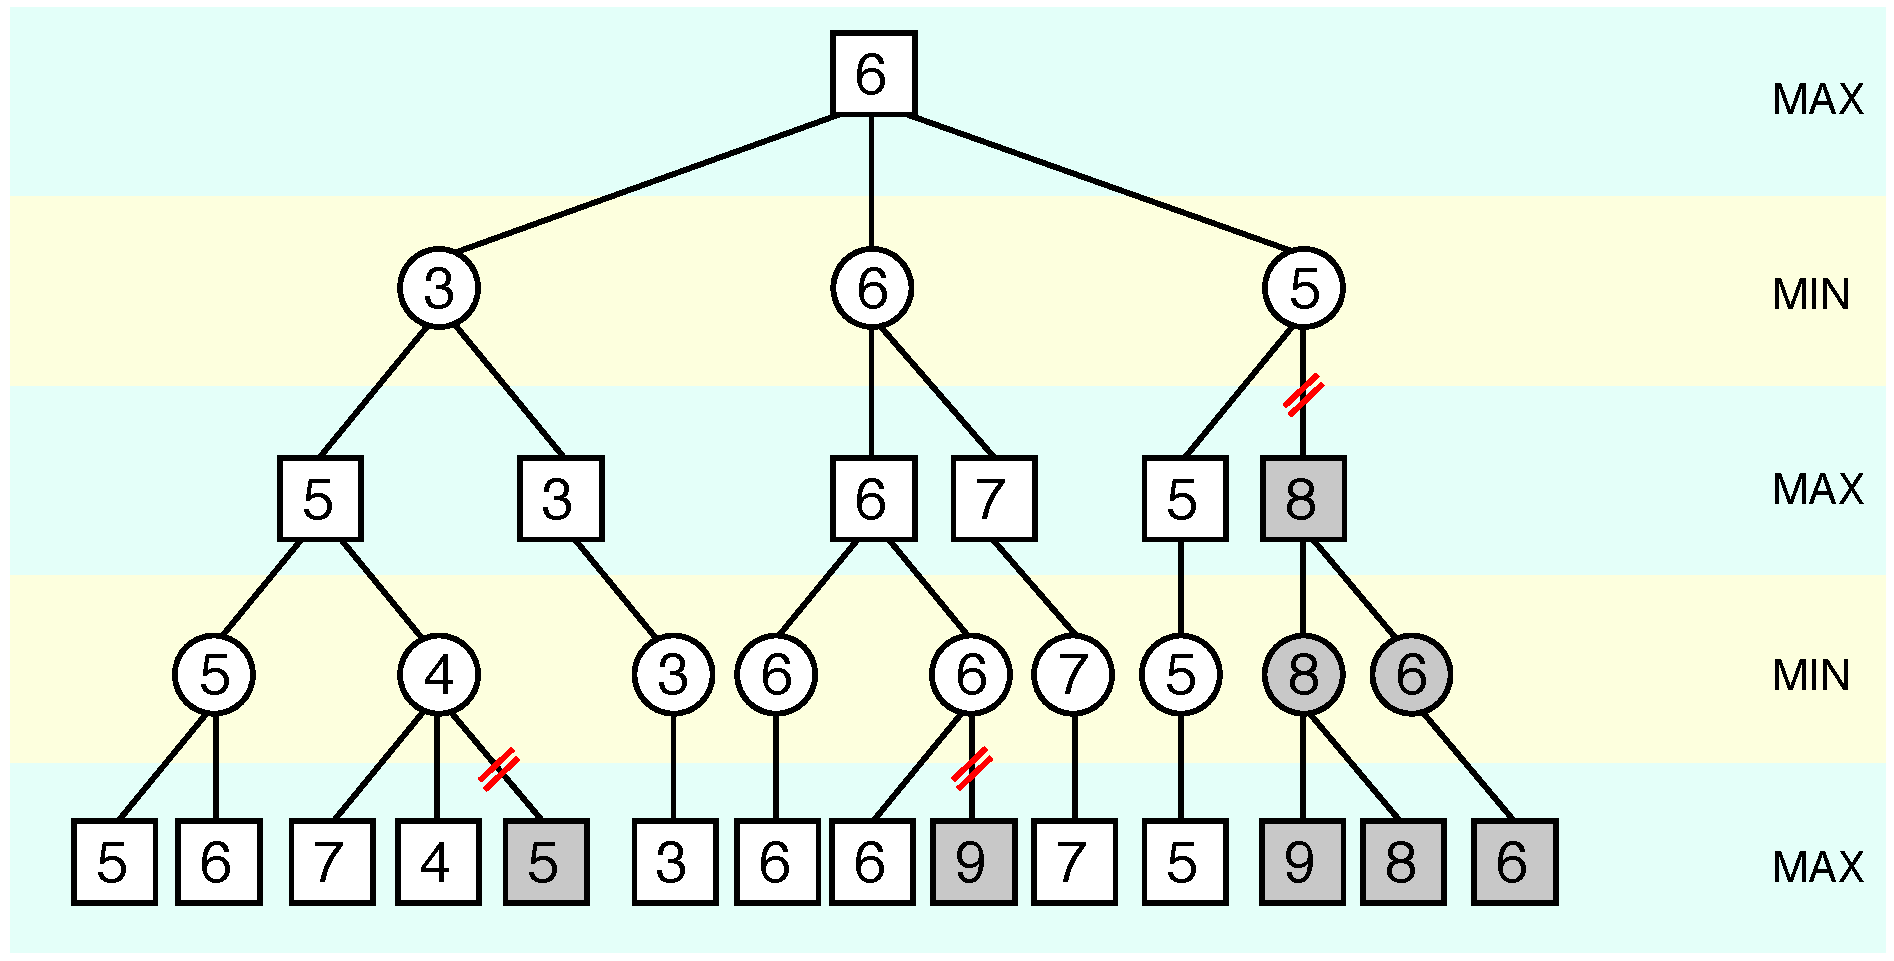
\epsfig{file=Figures/alpha-beta-pruning.pdf, scale=0.4}    
  \end{center}
  \caption{Example game tree showing $\alpha$-$\beta$-Pruning.
    (Original: \href{https://commons.wikimedia.org/wiki/File:AB_pruning.svg}{Wikipedia}.)}
\label{fig:alpha-beta-pruning.pdf}
\end{figure}

If we look at the game tree in Figure \ref{fig:alpha-beta-pruning.pdf} on page
\pageref{fig:alpha-beta-pruning.pdf} we notice that some numbers are greyed out.  The reason is that these
numbers can not influence the result of the game.  If we would replace these numbers with any arbitrary
numbers, the overall result of the game would not change if both players play optimally.
\begin{enumerate}
\item Let us first take a look at the greyed out node that is marked with a 5 in the bottom-most line.  This is the
      result value of a move from the player \texttt{Min}.   The parent of this node is marked with a 4.  In
      this node it is the turn of the player \texttt{Min}, who will choose the smallest possible value.  If the 5
      would be replaced by a 0, then \texttt{Min} would choose this zero.  This would change the node of the
      parent node, which currently is 4, to be 0.  However, this would not change the result of the game because
      in the parent of the node that is currently marked with a 4 it is the turn of \texttt{Max} and
      \texttt{Max} will choose the move leading to his left child because that already guarantees him the value 5.

      Similarly, if the value of the greyed out node was 10 instead of 5, the player \texttt{Min} would not
      choose this node because for her the node marked with 4 is a better choice.  Hence the value of the node
      currently marked with a 5 is of no consequence for the overall value of the game and therefore there is no
      need to evaluate this node at all.
\item The situation is similar for the first node marked with a greyed out 9 in the bottom-most line, because
      in the grandparent of this node it is the turn of the player \texttt{Max} and \texttt{Max} is already
      guaranteed the value of 6 at this node when he chooses the move leading to its left child.
\item At the right part of the tree we have a whole subtree that is greyed out.  The root of this subtree is
      marked with the number 8.  Let us understand the reason this subtree does not influence the value of the
      overall tree.
      \begin{enumerate}[(a)]
      \item The left sibling of the root node of the greyed out tree is marked with a 5. At the parent of this
            node, it is the turn of the player \texttt{Min}.  As \texttt{Min} can already choose the node
            labelled with a 5, we know that the parent node has a value that is at most five.
      \item However, the grandparent of this node is the root of the complete tree.  In this node, it is the
            turn of the player \texttt{Max}.  \texttt{Max} can achieve the value 6 by choosing his second child.
            Therefore the value of this node at least 6.  
      \item As we have already seen that the value of the rightmost child of the root node can be at most 5,
            \texttt{Max} will never choose this child, but will choose his second child instead.
      \end{enumerate}
      Therefore, the subtree whoose root is marked with a greyed out 8 does not influence the outcome of the game.
\end{enumerate}
To implement $\alpha$-$\beta$-pruning, the basic idea is to provide two additional arguments to the functions
$\textts{maxValue}$ and $\textts{minValue}$.  Traditionally, these arguments are called $\blue{\alpha}$ and $\blue{\beta}$.  In order to be able to
distinguish between the old functions $\textts{maxValue}$ and  $\textts{minValue}$ and its
improved version, we call the improved versions  
$\textts{alphaBetaMax}$ and $\textts{alphaBetaMin}$.  The idea is that these functions are
related by the following requirements: 
\begin{enumerate}
\item As long as $\textts{maxValue}(s)$ is between $\alpha$ and $\beta$, the function
      $\textts{alphaBetaMax}$ computes the same result as the function $\textts{maxValue}$,
      i.e.~we have
      \\[0.2cm]
      \hspace*{0.3cm}
      $\alpha \leq \textts{maxValue}(s) \leq \beta \;\rightarrow\;
         \textts{alphaBetaMax}(s, \alpha, \beta) = \textts{maxValue}(s)
      $.
\item If $\textts{maxValue}(s) < \alpha$, we require that the value returned by
      $\textts{alphaBetaMax}$ is less than or equal to $\alpha$, i.e.~we have 
      \\[0.2cm]
      \hspace*{0.3cm}
      $\textts{maxValue}(s) < \alpha \;\rightarrow\; \textts{alphaBetaMax}(s, \alpha, \beta) \leq \alpha$.
\item Similarly, if $\textts{maxValue}(s) > \beta$, we require that the value
      returned by $\textts{alphaBetaMax}$ is bigger than or equal to $\beta$, i.e.~we have 
      \\[0.2cm]
      \hspace*{0.3cm}
      $\beta < \textts{maxValue}(s) \;\rightarrow\; \beta \leq \textts{alphaBetaMax}(s, \alpha, \beta)$.
\end{enumerate}
Similar to the way that the function \textts{maxValue} is approximated by the function \textts{alphaBetaMax},
the function \textts{minValue} is approximated by the function \textts{alphaBetaMin}.  We have: 
\begin{enumerate}
\item $\alpha \leq \textts{minValue}(s) \leq \beta \;\rightarrow\;
         \textts{alphaBetaMin}(s, \alpha, \beta) = \textts{minValue}(s)
      $.
\item $\textts{minValue}(s) < \alpha \;\rightarrow\; \textts{alphaBetaMin}(s, \alpha, \beta) \leq \alpha$.
\item $\beta < \textts{minValue}(s) \;\rightarrow\; \beta \leq \textts{alphaBetaMin}(s, \alpha, \beta)$.
\end{enumerate}
Although $\textts{alphaBetaMax}(s)$and $\textts{alphaBetaMin}(s)$  are only \blue{approximations} of
$\textts{maxValue}(s)$ and $\textts{minValue}(s)$, it turns out that these approximations are all that
is needed.  Once the function $\textts{alphaBetaMax}$ is implemented, the function
$\textts{maxValue}$ can then be computed as 
\\[0.2cm]
\hspace*{1.3cm}
$\textts{maxValue}(s) := \textts{alphaBetaMax}(s, -1, +1)$.
\\[0.2cm]
The reason is that we already know that $-1 \leq \textts{maxValue}(s) \leq +1$ and hence the first case of the
specification of $\textts{alphaBetaMax}$ guarantees that the equation
\\[0.2cm]
\hspace*{1.3cm}
$\textts{maxValue}(s) = \textts{alphaBetaMax}(s,-1,+1)$
\\[0.2cm]
holds.  Similarly, the function $\textts{minValue}$ can be computed as 
\\[0.2cm]
\hspace*{1.3cm}
$\textts{minValue}(s) := \textts{alphaBetaMin}(s, -1, +1)$.
\\[0.2cm]
\myFig{Alpha-Beta-Pruning.ipynb:alphaBeta} shows an implementation of the functions $\textts{alphaBetaMax}$ and
$\textts{alphaBetaMin}$ that satisfies the specification given above.
Since $\textts{alphaBetaMax}$ and $\textts{alphaBetaMin}$ are implemented as mutually recursive functions, 
the fact that the implementations of $\textts{alphaBetaMax}$ and \textts{alphaBetaMin}
satisfy the specifications given above can be established by computational induction.
We proceed perform this proof.  The first proof of the correctness of $\alpha$-$\beta$-pruning has been given
by Donald E.~Knuth and Ronald W.~Moore \cite{knuth:1975}.


\begin{figure}[!ht]
\centering
\begin{python3code}
def alphaBetaMax(State, alpha, beta):
    if finished(State):
        return utility(State)
    for ns in next_states(State, gPlayers[0]):
        value = alphaBetaMin(ns, alpha, beta)
        if value >= beta:
            return value
        alpha = max(alpha, value)
    return alpha

def alphaBetaMin(State, alpha, beta):
    if finished(State):
        return utility(State)
    for ns in next_states(State, gPlayers[1]):
        value = alphaBetaMax(ns, alpha, beta)
        if value <= alpha:
            return value
        beta = min(beta, value)
    return beta
\end{python3code}
\caption{$\alpha$-$\beta$-Pruning.}
\label{fig:Alpha-Beta-Pruning.ipynb:alphaBeta}
\end{figure}

\noindent
We proceed to discuss the implementation of the function $\textts{alphaBetaMax}$, which is shown in
\myFig{Alpha-Beta-Pruning.ipynb:alphaBeta}.
\begin{enumerate}
\item If $\textts{State}$ is a terminal state, the function returns the $\textts{utility}$ of the given
      $\textts{State}$.
\item We iterate over all successor states $\textts{ns} \in \textts{next\_states}(\textts{State}, \textts{gPlayers}[0])$.
\item We have to recursively evaluate the states $\textts{ns}$ with respect to the minimizing player
      \textts{gPlayers[1]}.  Hence we call the function $\texttt{alphaBetaMin}$ when evaluating
      the state $\mathtt{ns}$.
\item As the specification of $\textts{alphaBetaMax}$ asks us to compute the value of $\textts{State}$ only in
      those cases where it is less than or equal to $\mathtt{beta}$, once we find a successor state $s$ that has a
      $\textts{value}$ that is at least as big as $\mathtt{beta}$ we can \blue{stop any further evaluation} of the successor
      states and return $\textts{value}$.

      This shortcut results in significant savings of computation time!
\item Once we have found a successor state that has a value $\textts{value}$ greater than $\textts{alpha}$,
      we can increase $\textts{alpha}$ to $\textts{value}$.  The reason is, that once we know we can
      achieve $\textts{value}$ we are no longer interested in any smaller values.
      This is the reason for assigning the maximum of $\textts{value}$ and $\textts{alpha}$ to $\textts{alpha}$.

      After this assignment, $\texttt{alpha}$ will be at least as big as $\texttt{value}$ and according to the specification
      of $\texttt{alphaBetaMax}$ we can therefore return $\texttt{alpha}$.
\end{enumerate}

\noindent
\textbf{Claim}: The functions \texttt{alphaBetaMax} and $\mathtt{alphaBetaMin}$ both satisfy the specification
given previously. 
\vspace*{0.2cm}

\noindent
\textbf{Proof}:  The proof proceeds by computational induction.  However, we will only show that
the function \texttt{alphaBetaMax} satisfies its specification, as the proof of the correctness of the function
\texttt{alphaBetaMin} is completely analogous to the proof of the correctness of \texttt{alphaBetaMax}.  Furthermore,
to simplify the proof we define $\mathtt{A} := \mathtt{gPlayers}[0]$ and $\mathtt{B} := \mathtt{gPlayers}[1]$.
\begin{enumerate}
\item[B.C:] $S \in \mathtt{TerminalStates}$, that is $\texttt{finished}(S) = \mathtt{True}$.

  In this case we have $\texttt{alphaBetaMax}(S, \alpha, \beta) = \texttt{utility}(S)$ and since in this case we also have
  $\texttt{maxValue}(S) = \texttt{utility}(S)$ this implies
  \\[0.2cm]
  \hspace*{1.3cm}
  $\texttt{alphaBetaMax}(s, \alpha, \beta) = \texttt{maxValue}(S)$.   \hspace*{\fill} $(*)$
  \\[0.2cm]
  We have to check the three cases of our specification one by one.
  \begin{enumerate}
  \item $\alpha \leq \mathtt{maxValue}(S) \leq \beta$.

        We have to show that $\texttt{alphaBetaMax}(s, \alpha, \beta) = \texttt{maxValue}(S)$ holds.
        This follows immediately from $(*)$.
  \item $\texttt{maxValue}(S) < \alpha$. Because of $(*)$ this implies
        \\[0.2cm]
        \hspace*{1.3cm}
        $\texttt{alphaBetaMax}(s, \alpha, \beta) < \alpha$
        \\[0.2cm]
        and therefore we also have $\texttt{alphaBetaMax}(S) \leq \alpha$.  
  \item $\beta < \mathtt{maxValue}(S)$.  Because of $(*)$ this implies
        \\[0.2cm]
        \hspace*{1.3cm}
        $\beta < \mathtt{alphaBetaMax}(s, \alpha, \beta)$
        \\[0.2cm]
        and therefore we also have $\beta \leq \mathtt{alphaBetaMax}(S, \alpha, \beta)$.
  \end{enumerate}
  This finishes the proof of the base case.
\item[I.S.:] This time $S\not\in \mathtt{TerminalStates}$.  As we have to check all three cases of our
  specification, we have to carry out a case distinction.
  \begin{enumerate}[(a)]
  \item $\alpha \leq \mathtt{maxValue}(S) \leq \beta$.

        We have to show that in this case $\mathtt{alphaBetaMax}(S) = \mathtt{maxValue}(S)$.
        There are two subcases.
        \begin{enumerate}
        \item If $\texttt{maxValue}(S) = \beta$ there has to be a node $\texttt{ns} \in \texttt{nextStates}(S,
          A)$ such that
              \\[0.2cm]
              \hspace*{1.3cm}
              $\texttt{minValue}(\mathtt{ns}) = \beta$.
              \\[0.2cm]
              When the \texttt{for}-loop hits this node, the
              condition of the \texttt{if}-statement in line 6 is true and the value of this node,
              which is $\beta$, is returned.   Therefore we have
              \\[0.2cm]
              \hspace*{1.3cm}
              $\texttt{alphaBetaMax}(S, \alpha, \beta) = \beta = \texttt{maxValue}(S)$.
        \item If $\texttt{maxValue}(S) < \beta$, then we know that for all states
              $\texttt{ns} \in \mathtt{nextStates}(S, \mathtt{B})$ we must have 
              \\[0.2cm]
              \hspace*{1.3cm}
              $\texttt{minValue}(\mathtt{ns}) < \beta$.              
              \\[0.2cm]
              From the specification and the induction hypothesis it the follows that
              \\[0.2cm]
              \hspace*{1.3cm}
              $\texttt{alphaBetaMin}(\mathtt{ns}, \alpha, \beta) < \beta$.              
              \\[0.2cm]
              Furthermore, since $\alpha \leq \mathtt{maxValue}(S)$ there must exists a state
              $\texttt{ns} \in \mathtt{nextStates}(S, \mathtt{A})$ such that
              \\[0.2cm]
              \hspace*{1.3cm}
              $\alpha \leq \mathtt{minValue}(\mathtt{ns})$
              \\[0.2cm]
              W.l.o.g.~assume that $\mathtt{ns}$ is the node with the maximal value, i.e.~we have
              \\[0.2cm]
              \hspace*{1.3cm}
              $\texttt{maxValue}(S) = \texttt{minValue}(\texttt{ns})$.
              \\[0.2cm]
              As we already know that $\texttt{minValue}(\texttt{ns}) < \beta$, the induction hypothesis tells us that 
              \\[0.2cm]
              \hspace*{1.3cm}
              $\texttt{alphaBetaMin}(\mathtt{ns}, \alpha, \beta) = \texttt{minValue}(\mathtt{ns})$
              \\[0.2cm]
              Hence the value computed in the \texttt{for}-loop is equal to
              $\mathtt{alphaBetaMin}(\mathtt{ns}, \alpha, \beta)$ and therefore we have
              \\[0.2cm]
              \hspace*{0.3cm}
              $\mathtt{alphaBetaMax}(S, \alpha, \beta) = \mathtt{alphaBetaMin}(\mathtt{ns}, \alpha, \beta)
              = \mathtt{minValue}(\mathtt{ns}) = \mathtt{maxValue}(S)$.
        \end{enumerate}
  \end{enumerate}
\item $\texttt{maxValue}(S) < \alpha$

  In this case we only have to show that $\mathtt{alphaBetaMax}(S, \alpha, \beta) \leq \alpha$.
  Since $\texttt{maxValue}(S) < \alpha$ it must be the case that
  \\[0.2cm]
  \hspace*{1.3cm}
  $\mathtt{minValue}(\mathtt{ns}) < \alpha$ \quad for all $\mathtt{ns} \in \mathtt{nextStates}(S)$.
  \\[0.2cm]
  By induction hypothesis this implies
  \\[0.2cm]
  \hspace*{1.3cm}
  $\mathtt{alphaBetaMin}(\mathtt{ns}, \alpha, \beta) \leq \alpha$ \quad for all $\mathtt{ns} \in \mathtt{nextStates}(S)$.
  \\[0.2cm]
  Since the \texttt{for}-loop computes the maximum of these values it follows that
  \\[0.2cm]
  \hspace*{1.3cm}
  $\mathtt{alphaBetaMax}(S, \alpha, \beta) \leq \alpha$. 
\item $\beta < \texttt{maxValue}(S)$

  In this case we have to show that $\beta \leq \mathtt{alphaBetaMax}(s, \alpha, \beta)$.
  The assumption $\beta < \texttt{maxValue}(S)$ implies that there is node
  $\texttt{ns} \in \texttt{nextStates}(S, \texttt{A})$ such that 
  \\[0.2cm]
  \hspace*{1.3cm}
  $\beta < \texttt{minValue}(\texttt{ns})$.
  \\[0.2cm]
  By induction hypothesis we can conclude that
  \\[0.2cm]
  \hspace*{1.3cm}
  $\beta \leq \mathtt{alphaBetaMin}(\mathtt{ns}, \alpha, \beta)$.
  \\[0.2cm]
  But then this value (or another one greater or equal than $\beta$) is returned by the \texttt{if}-statement
  in line 6 and hence we have
  \\[0.2cm]
  \hspace*{1.3cm}
  $\beta \leq \mathtt{alphaBetaMax}(S, \alpha, \beta)$.
\end{enumerate}
As the function \texttt{alphaBetaMax} satisfies its specification in all three cases, the proof is complete. \qed

\remark
There is a nice simulator for alpha-beta-pruning available at the following web address:
\href{https://pascscha.ch/info2/abTreePractice/}{https://pascscha.ch/info2/abTreePractice/}.

\exercise
The game \href{https://en.wikipedia.org/wiki/Nim}{Nim} works as follows:
\begin{enumerate}[(a)]
\item There are four rows of matches:
      \begin{enumerate}[1.]
      \item the first  row contains 1 match,
      \item the second row contains 3 matches,
      \item the third  row contains 5 matches, and
      \item the fourth row contains 7 matches.
     \end{enumerate}
\item The player whose turn it is first selects a line.
     
      Then she removes any number of matches from this line.
\item The player that removes the last match has won the game. 
\end{enumerate}
Implement this game by adapting the notebook
\\[0.2cm]
\hspace*{1.3cm}
\href{https://github.com/karlstroetmann/Artificial-Intelligence/blob/master/Python/3 Games/Nim-Frame.ipynb}{
   Artificial-Intelligence/blob/master/Python/3 Games/Nim-Frame.ipynb}.
\\[0.2cm]
 Then,  test the game using the notebook
\\[0.2cm]
\hspace*{1.3cm}
\href{https://github.com/karlstroetmann/Artificial-Intelligence/blob/master/Python/3 Games/5-Alpha-Beta-Pruning.ipynb}{Artificial-Intelligence/blob/master/Python/3 Games/5-Alpha-Beta-Pruning.ipynb}.
\eox


\subsection{Alpha-Beta Pruning with Memoization}
Adding memoization to the functions \textts{maxValue} and \textts{minValue} is non-trivial.
If memoization is added in a naive way, then the cache might have many entries for the same state that differ
only in their values for the parameters $\alpha$ and $\beta$.  Although this is not a problem for trivial games
like Tic-Tac-Toe, it becomes a problem once we try to implement more complex games like
\href{https://en.wikipedia.org/wiki/Connect_Four}{Connect Four}. The reason is that for those games we are no
longer able to compute the complete game tree.  Instead, we need to approximate the value of a state with the
help of a heuristic.  Then, $\alpha$ and $\beta$ will no longer be confined to the values from the set
$\{-1,0,1\}$ but will rather take on a continuous set of values from the interval $[-1, +1]$.  Hence there will
be many function calls of the form 
\\[0.2cm]
\hspace*{1.3cm}
$\textts{maxValue}(s, \alpha, \beta)$ 
\\[0.2cm]
where the state $s$ is the same but $\alpha$ and $\beta$ are different.  If we would try to store every
combination of $s$, $\alpha$, and $\beta$ we would waste a lot of memory and, furthermore, we would have only a
small number of cache hits.  Therefore, we will now present a more effective way to cache the functions
\textts{maxValue} and \textts{minValue}.  The method we describe here is an adaption of the method published by
Marsland and Campbell \cite{marsland:82}.
To this end we will define a function \textts{evaluate} that is
called as follows:
\\[0.2cm]
\hspace*{1.3cm}
$\textts{evaluate}(s, f, \alpha, \beta)$
\\[0.2cm]
where the parameters are interpreted as follows:
\begin{enumerate}[(a)]
\item $s$ is a state that is to be evaluated.
\item $f$ is either the function \textts{alphaBetaMax} or the function \textts{alphaBetaMin}.
      If in state $s$ the first player has to move, then $f = \textts{alphaBetaMax}$, otherwise we have
      $f = \textts{alphaBetaMin}$.
\item We interpret the parameters $\alpha$ and $\beta$ in the same way as we did when we used them with
      the functions $\textts{alphaBetaMax}$ and $\textts{alphaBetaMin}$.
\end{enumerate}
The function \textts{evaluate} encapsulates calls to the functions \texttt{alphaBetaMax} and
\texttt{alphaBetaMin}.  Given a state $s$, a function $f$, and the values of $\alpha$ and $\beta$, 
it first checks whether the value of $f(s, \alpha, \beta)$ has already been computed and is stored in the
cache.  If this is the case, the value is returned.  Otherwise, the function $f$ is called.  

The function \textts{evaluate} makes use of a global variable \textts{gCache}.  This variable is used as a
cache to store the results of the function \textts{evaluate}.  This cache is implemented as a dictionary.  The
keys of this dictionary are the just the states, not triples of the form $\langle s, \alpha, \beta \rangle$.  The values
stored in the cache are pairs of the form $(\textts{flag}, v)$, where $v$ is a value computed by the
function $\textts{evaluate}(s, f, \alpha, \beta)$, while $\textts{flag}$ specifies whether $v$ is exact, a
lower bound, or an upper bound.  We have
\\[0.2cm]
\hspace*{1.3cm}
$\textts{flag} \in \{ \quoted{\leq}, \quoted{=}, \quoted{\geq}\}$.
\\[0.2cm]
The cache satisfies the following specification:
\begin{enumerate}
\item $\texttt{gCache}[s] = (\quoted{=}, v) \rightarrow f(s, \alpha, \beta) = v$

      If the flag is equal to \quoted{=}, then the value stored in $\textts{gCache}[s]$
      is the \blue{exact} value computed for the given state $s$ by the function $f$.
\item $\texttt{gCache}[s] = (\quoted{\leq}, v) \rightarrow f(s, \alpha, \beta) \leq v$

      If the flag is equal to \quoted{\leq}, then the value stored in $\textts{gCache}[s]$
      is an \blue{upper bound} for the value returned from $f(s, \alpha, \beta)$.  

\item $\texttt{gCache}[s] = (\quoted{\geq}, v) \rightarrow f(s, \alpha, \beta) \geq v$

      If the flag is equal to \quoted{\geq}, then the value stored in \textts{gCache[State]}
      is a \blue{lower bound} for $f(s, \alpha, \beta)$.
\end{enumerate}
If $\textts{gCache}[s]$ is defined, then the computation of $\texttt{evaluate}(s, f, \alpha, \beta)$
proceeds according to the following case distinction:
\begin{enumerate}
\item If the stored value $v$ is exact, we can return this value:
      \\[0.2cm]
      \hspace*{1.3cm}
      $\texttt{gCache}[s] = (\quoted{=}, v) \rightarrow \texttt{evaluate}(s, f, \alpha, \beta) = v$.
\item If the stored value $v$ is an upper bound, then there are two cases.
      \begin{enumerate}[(a)]
      \item If this upper bound $v$ is less or equal than $\alpha$, then we know that
            the true value of the state $s$ is less or equal than $\alpha$ and hence we can also return the value $v$:
            \\[0.2cm]
            \hspace*{1.3cm}
            $\texttt{gCache}[s] = (\quoted{\leq}, v) \wedge v \leq \alpha \rightarrow 
     \texttt{evaluate}(s, f, \alpha, \beta) = v$.
      \item Otherwise we can sharpen the upper bound $\beta$ by setting $\beta$ to be the minimum of $\beta$
            and $v$:
            \\[0.2cm]
            \hspace*{1.3cm}
            $\texttt{beta} = \texttt{min}(\texttt{beta}, v)$.
            \\[0.2cm]
            If this leads to a reduction of $\beta$, then size of the interval $[\alpha, \beta]$ is reduced
            and hence Alpha-Beta pruning will be able to remove more nodes from the game tree, making the
            search more efficient.
      \end{enumerate}
      \item If the stored value $v$ is a lower bound, there are again two cases.
      \begin{enumerate}
      \item If this lower bound is greater or equal than $\beta$, then we 
            know that the true value is bigger or equal than $\beta$ and hence we can return the value $v$: 
            \\[0.2cm]
            \hspace*{1.3cm}
            $\texttt{gCache}[s] = (\quoted{\geq}, v) \wedge \beta \leq v \rightarrow 
     \texttt{evaluate}(s, f, \alpha, \beta) = v$.
      \item Otherwise, we can sharpen the lower bound $\alpha$ by setting $\alpha$ to be the maximum of
            $\alpha$ and $v$:
            \\[0.2cm]
            \hspace*{1.3cm}
            \texttt{alpha} = \texttt{max}(\texttt{alpha}, v)
            \\[0.2cm]
            If this leads to an increase of $\alpha$, then size of the interval $[\alpha, \beta]$ is reduced
            and hence Alpha-Beta pruning will be able to remove more nodes from the game tree, making the
            search more efficient.
      \end{enumerate}
\end{enumerate}
Finally, we call the function $f$ on the given state with lower bound $\alpha$ and upper bound $\beta$ and
store the value that is computed in the cache via the function \texttt{store\_cache}.  This function has to
store both the value and the appropriate flag.

\begin{figure}[!ht]
\centering
\begin{minted}[ frame         = lines, 
                framesep      = 0.3cm, 
                firstnumber   = 1,
                bgcolor       = sepia,
                numbers       = left,
                numbersep     = -0.2cm,
                xleftmargin   = 0.0cm,
                xrightmargin  = 0.0cm,
              ]{python3}
    def evaluate(State, f, alpha=-1, beta=1):
        global gCache
        if State in gCache:
            flag, v = gCache[State]
            if flag == '=':
                return v
            if flag == '<=':
                if v <= alpha:
                    return v
                else:
                    beta = min(beta, v)
            if flag == '>=':
                if beta <= v:
                    return v
                else:
                    alpha = max(alpha, v)
        v = f(State, alpha, beta)
        store_cache(State, alpha, beta, v)
        return v

    def store_cache(State, alpha, beta, v):
        global gCache
        if   v <= alpha:
            gCache[State] = ('<=', v)
        elif v <  beta: # alpha < v
            gCache[State] = ('=', v)
        else: # beta <= v
            gCache[State] = ('>=', v)            
\end{minted}
\vspace*{-0.3cm}
\caption{Implementation of the function \texttt{evaluate}.}
\label{fig:evaluate}
\end{figure}
\FloatBarrier

\begin{figure}[!ht]
\centering
\begin{python3code}
def maxValue(State, alpha, beta):
    if finished(State):
        return utility(State)
    for ns in next_states(State, gPlayers[0]):
        value = evaluate(ns, minValue, alpha, beta)
        if value >= beta:
            return value
        alpha = max(alpha, value)
    return alpha

def minValue(State, alpha, beta):
    if finished(State):
        return utility(State)
    for ns in next_states(State, gPlayers[1]):
        value = evaluate(ns, maxValue, alpha, beta)
        if value <= alpha:
            return value
        beta = min(beta, value)
    return beta    
\end{python3code}
\vspace*{-0.3cm}
\caption{Cached implementation of the functions \texttt{alphaBetaMax} and \texttt{alphaBetaMin}.}
\label{fig:alphaBetaCached}
\end{figure}
\FloatBarrier

\section{Progressive Deepening}
In practice, most games are far too complex to be evaluated completely, i.e.~the size of the set
$\textts{States}$ is so big that even the fastest computer does not stand a chance to explore this set
completely.  For example, it is believed\footnote{
  For reference, compare the wikipedia article on the so-called
  \href{https://en.wikipedia.org/wiki/Shannon_number}{Shannon number}.
  The Shannon number estimates that there are at least $10^{120}$ different plays in chess.  However, the
  number of states is estimated to be about $(4.48\pm 0.37) \cdot 10^{44}$. 
}
that in chess there are about $4.48 \cdot 10^{44}$ different states that could occur in a game.
Hence, it is impossible to explore all possible states in chess.  Instead, we have to limit
the exploration in a way that is similar to the way professional players evaluate their games:  Usually, a
player considers all variations of a game for, say, the next three moves.  After a given number of moves, the
value of a position is estimated using an \blue{evaluation heuristic}.  This function \blue{approximates} the true
value of a given state via a heuristic.

\begin{figure}[!ht]
\centering
\begin{minted}[ frame         = lines, 
                  framesep      = 0.3cm, 
                  firstnumber   = 1,
                  bgcolor       = sepia,
                  numbers       = left,
                  numbersep     = -0.2cm,
                  xleftmargin   = 0.0cm,
                  xrightmargin  = 0.0cm,
                ]{python3}
    def pd_evaluate(State, limit, f=maxValue):
        for l in range(limit+1):
            value = evaluate(State, l, f)
            if value in [-1, 1]:
                return value
        return value
\end{minted}
\caption{Progressive Deepening}
\label{fig:Game.ipynb:pd_evaluate}
\end{figure}
\FloatBarrier


In order to implement this idea, we add a parameter $\textts{limit}$ to the procedures $\textts{alphaBetaMax}$
and $\textts{alphaBetaMin}$ that were shown in the previous section.  On
every recursive invocation of the functions $\textts{alphaBetaMax}$ and $\textts{alphaBetaMin}$, the parameter
$\textts{limit}$ is decreased. 
Once the limit reaches $0$, instead of invoking the function $\textts{alphaBetaMax}$ or $\textts{alphaBetaMin}$
again, we try to estimate the value of the given $\textts{State}$ using an \blue{evaluation heuristic}.  This
leads to the code shown in \myFig{Game.ipynb}. 

When we compare this Figure with \myFig{Alpha-Beta-Pruning.ipynb:alphaBeta}, the only difference is in line 4
where we test whether the $\textts{limit}$ is $0$.  In this case, instead of trying to recursively evaluate the
states reachable from $\textts{State}$, we evaluate the $\textts{State}$ with a $\textts{heuristic}$ function
that tries to guess the approximate value of a given state.
Notice that in the calls of the function \textts{evaluate} we have to take care to decrease the parameter
$\textts{limit}$.  The function $\textts{evaluate}$ is responsible for administering the cache as previously.

\begin{figure}[!ht]
\centering
\begin{minted}[ frame         = lines, 
                  framesep      = 0.3cm, 
                  firstnumber   = 1,
                  bgcolor       = sepia,
                  numbers       = left,
                  numbersep     = -0.2cm,
                  xleftmargin   = 0.0cm,
                  xrightmargin  = 0.0cm,
                ]{python3}
    def maxValue(State, limit, alpha=-1, beta=1):
        if finished(State):
            return utility(State)
        if limit == 0:
            return heuristic(State)
        value      = alpha
        NextStates = next_states(State, gPlayers[0])
        Moves      = []  # empty priority queue
        for ns in NextStates:
            val = value_cache(ns, limit-2) 
            if val == None:
                val = -1 # unknown values are assumed to be worse than known values
            # heaps are sorted ascendingly, hence the minus
            heapq.heappush(Moves, (-val, ns))
        while Moves != []:
            _, ns = heapq.heappop(Moves)
            value = max(value, evaluate(ns, limit-1, minValue, value, beta))
            if value >= beta:
                return value
        return value
    
    def minValue(State, limit, alpha=-1, beta=1):
        if finished(State):
            return utility(State)
        if limit == 0:
            return heuristic(State)
        value      = beta
        NextStates = next_states(State, gPlayers[1])
        Moves      = []  # empty priority queue
        for ns in NextStates:
            val = value_cache(ns, limit-2)
            if val == None:
                val = 1
            heapq.heappush(Moves, (val, ns))
        while Moves != []:
            _, ns = heapq.heappop(Moves)
            value = min(value, evaluate(ns, limit-1, maxValue, alpha, value))
            if value <= alpha:
                return value
        return value
    
        def value_cache(State, limit):
        flag, value = gCache.get((State, limit), ('?', None))
            return value
\end{minted}
\caption{Depth-limited $\alpha$-$\beta$-pruning.}
\label{fig:Game.ipynb}
\end{figure}

There is one further difference between the functions $\textts{maxValue}$ and $\textts{minValue}$ shown in
Figure \ref{fig:Game.ipynb} and those versions of these functions that were shown previously:
In Figure \ref{fig:Game.ipynb} the $\textts{NextStates}$ are stored in a priority queue such that the move that
is considered to be the best has the highest priority.  This way, the best moves are tried first and as a
result alpha-beta-pruning is able to prune larger parts of the search space.
In order to guess which move is best we use the cached values of the corresponding states.  This is the real
reason for using progressive deepening:  When we evaluate the states with a depth limit of $l$, we can use the
values of the states that has been stored previously when those states were evaluated with a depth limit of
$l-2$.  At this point the reader might be surprised: Wouldn't the value computed for a depth limit of $l-1$ be
more accurate than the value for a depth limit of $l-2$?  The answer is no.  This can be both verified
experimentally and explained theoretically.  To understand why the value for the depth of $l-2$ is better than
the value for $l-1$, let us think about the game of chess.  Assume first that we have a depth limit of $1$,
i.e. we look only one half move into the future.  This would result in very aggressive play, i.e.~the computer
would always try to capture a piece if possible.  For example, if the only capture possible would be the queen
capturing a  pawn, the computer would take this pawn, even if it would loose the queen in the following move
because a look ahead depth of 1 is just not sufficient.  With a depth limit of $2$ the computer would play more
defensive. However, when the depth is incremented to 3, the computer would play more aggressive again.
Although it would then not sacrifice a queen to capture a pawn, it still would prepare to capture a pawn with
the queen in its second move.  For this reason, it is usually best to have a depth limit that is even, because
if the depth limit is odd, the computer would play too aggressive as it would not be able to see the way in
which his last move is answered by its opponent.  Therefore, the values stored for a depth limit of $l-2$ are
actually better than those for a depth limit of $l-1$. 


For a game like tic-tac-toe it is difficult to come up with a decent heuristic.  A very crude approach would be
to define:
\\[0.2cm]
\hspace*{1.3cm}
\textts{heuristic := [State, player] |-> 0;}
\\[0.2cm]
This heuristic would simply estimate the value of all states to be $0$.  As this heuristic is only called after
it has been tested that the game has not yet been decided, this approach is not utterly unreasonable.  For a more
complex game like chess, the heuristic could instead be a \blue{weighted count} of all pieces.  Concretely, the
algorithm for estimating the value of a state would work as follows:
\begin{enumerate}
\item Initially, the variable $\textts{sum}$ is set to $0$:
      \\[0.2cm]
      \hspace*{1.3cm}
      \textts{sum := 0;}
\item We would count the number of white rooks $\textts{Rook}_{\mathrm{white}}$ and black rooks $\textts{Rook}_{\mathrm{black}}$,
      subtract these numbers from each other and multiply the difference by $5$.  
      The resulting number would be added to $\textts{sum}$:
      \\[0.2cm]
      \hspace*{1.3cm}
      $\textts{sum} \;\textts{+=}\; (\textts{Rook}_{\mathrm{white}} - \textts{Rook}_{\mathrm{black}}) \cdot 5\textts{;}$
\item We would count the number of white bishops $\textts{Bishop}_{\mathrm{white}}$ and black bishops
      $\textts{Bishop}_{\mathrm{black}}$,
      subtract these numbers from each other and multiply the difference by $3$.  
      The resulting number would be added to $\textts{sum}$:
      \\[0.2cm]
      \hspace*{1.3cm}
      $\textts{sum} \;\textts{+=}\; (\textts{Bishop}_{\mathrm{white}} - \textts{Bishop}_{\mathrm{black}}) \cdot 3\textts{;}$
\item In a similar way we would count knights, queens, and pawns.  Approximately, the weights of
      knights are $3$, a queen is worth $9$ and a pawn is worth $1$.
\end{enumerate}
The resulting $\textts{sum}$ can then be used as an approximation of the value of a state.
More details about the weights of the pieces can be found in the Wikipedia article 
``\href{https://en.wikipedia.org/wiki/Chess_piece_relative_value}{chess piece relative value}''.

% \exercise
% The game \blue{three men's morris} is described in the following YouTube video:
% \\[0.2cm]
% \hspace*{1.3cm}
% \href{https://www.youtube.com/watch?v=R-aSW1MQwEo}{\textts{https://www.youtube.com/watch?v=R-aSW1MQwEo}}
% \\[0.2cm]
% The game is played on a board of size $3 \times 3$, i.e.~it is played on the same board as tic-tac-toe.
% There are two players, which we will call \textts{X} and \textts{O}.  The bottom row of the board is filled
% with three coins that are marked with an \textts{'X'} on top, while the top row is filled with three coins that
% are marked with an \textts{'O'} on top.  The coins marked with an \textts{'X'} are assigned to the player \textts{X},
% while the coins marked with an \textts{'O'} are assigned to player \textts{O}.
% On each turn, the player whose turn it is moves one of his coins into an adjacent empty field.  The coins can be
% moved vertically, horizontally, and diagonally. 
% Player \textts{X} starts.  The goal of the game for player \textts{X} is to get three \textts{X}s into a row, column, or
% diagonal line, while player \textts{O} needs to get three \textts{O}s into a row, column, or diagonal line.  However, for
% player \textts{X} filling the bottom row with \textts{'X'}s does not count as a victory, while for player
% \textts{O}  filling the top row with \textts{'O'}s does not count as a victory.
% \begin{enumerate}[(a)]
% \item Implement this game by adapting the notebook
%       \\[0.2cm]
%       \hspace*{1.3cm}
%       \href{https://github.com/karlstroetmann/Artificial-Intelligence/blob/master/Python/3 Games/Tic-Tac-Toe.ipynb}{
%             Artificial-Intelligence/blob/master/Python/3 Games/Tic-Tac-Toe.ipynb}
%       \\[0.2cm]
%       from my GitHub page \textts{https://github.com/karlstroetmann}.
% \item Test the game using the notebook
%       \\[0.2cm]
%       \hspace*{1.3cm}
%       \href{https://github.com/karlstroetmann/Artificial-Intelligence/blob/master/Python/3 Games/Game-Move-Ordering.ipynb}{
%            Artificial-Intelligence/blob/master/Python/3 Games/Game-Move-Ordering.ipynb}.
%       \eox
% \end{enumerate}
% \pagebreak

\exercise
Read up on the game \href{https://en.wikipedia.org/wiki/Connect_Four}{Connect Four}.  You can play it online at
\\[0.2cm]
\hspace*{1.3cm}
\href{https://connect4.gamesolver.org/en/}{\textts{https://connect4.gamesolver.org/en/}}
\\[0.2cm]
Your task is to implement this game.  On my github page (\textts{https://github.com/karlstroetmann}) at
\\
\hspace*{1.3cm}
\href{https://github.com/karlstroetmann/Artificial-Intelligence/blob/master/Python/3
  Games/Connect-Four-Frame.ipynb}{Artificial-Intelligence/blob/master/Python/3 Games/Connect-Four-Frame.ipynb} 
\\[0.2cm]
is a frame  that can be used to solve this exercise.  
Once you have a running implementation of \blue{Connect Four}, try to improve the strength of your program by
adding a non-trivial heuristic to evaluate non-terminal states.  As an example of a non-trivial heuristic you
can define a \blue{triple} as a set of three marks of either \textts{X}s or \textts{O}s in a row that is
followed by a blank space.  The blank space could also be between the marks.  Now if there is a state $s$ that
has $a$ triples of \textts{X}s and $b$ triples of \textts{O}s and the game is not finished, then define
\\[0.2cm]
\hspace*{1.3cm}
$\ds \textts{value}(s, \textts{X}, \textts{limit}, \alpha, \beta) = \frac{a - b}{10}$ \quad if $\textts{limit} = 0$.
\eox

%%% Local Variables:
%%% mode: latex
%%% TeX-master: "artificial-intelligence"
%%% End:
